The experimental setup will be described in this section. Three models will be evaluated, Isolation Forest on the original data before compression, Isolation Forest on the compressed data and the proposed DupRes Isolation Forest on the compressed data. We will refer the different model in the same order as, \textbf{original}, \textbf{bases} and \textbf{DupRes}. The models are evaluated on various datasets containing anomalies. The datasets are described in the following subsections.

\subsection*{Synthetic}
The synthetic dataset is self-generated. It is two dimensional where each feature is an integer. The dataset contains three clusters where the samples are normally distributed with a standard deviation of 2, $N(\mu, 2^2)$ where $\mu$ varies on the cluster center. The data set is represented before and after compression on Figure \ref{fig:synthetic-dataset}. Each cluster consists of 150 samples and 20 outliers are generated between the clusters. There is then a total of 470 samples.

\begin{figure}
  \centering
  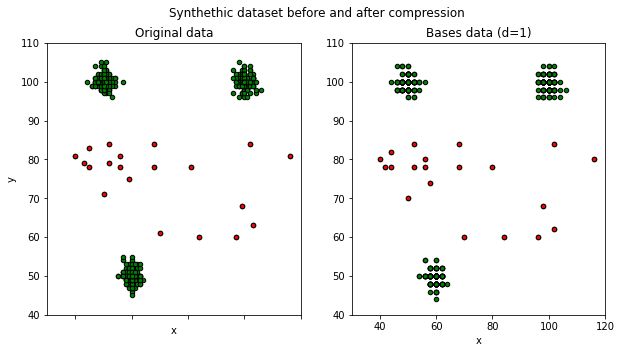
\includegraphics[width=\linewidth]{images/synthethic-dataset.png}
  \caption{Synthetic data set before(left) and after(right) compression with 1 deviation bit. Green points are inliers, while the red are outliers. }
  \label{fig:synthetic-dataset}
\end{figure}

\subsection*{Pendigits}
Pendigts is a database for handwritten digits. Originally it contains 16 integer features  with 10 classes (one for each digit). The dataset's 6870 samples is mapped to inliers and outliers to be utilized for anomaly detection \cite{ODDS}.

\subsection*{Shuttle}
The shuttle dataset contains 49097 samples collected from a shuttle. It has 9 dimensions all being integers \cite{ODDS}.

\subsection*{Waveform}
Waveform contains 3443 samples with 100 outliers. It has 21 features that are all numeric \cite{waveform}.

\subsection*{WBC}
The WBC dataset contains data of measurements from breast cancer cases. The inliers is the benign class, while the outliers are the malignant class. It contains 278 samples with 30 dimensions \cite{ODDS}.

\subsection{Preprocessing}
All of the features of the synthetic, pendigits and shuttle datasets can be represented as an one byte integer. However, the WBC and waveform datasets contains floating numbers. Therefore, the features are scaled with a factor of 10.

\subsection{Procedure}
The experiments is realized in Python and can be found for replication on github\footnote{\href{https://github.com/mlRosenquist/au-mlr-research-and-development-dedup}{https://github.com/mlRosenquist/au-mlr-research-and-development-dedup}}. DupRes is implemented by extending \textit{sklearn}'s existing Isolation Forest functionality. Thus, a fork is as well to be found on github\footnote{\href{https://github.com/mlRosenquist/scikit-learn}{https://github.com/mlRosenquist/scikit-learn}}.
Each dataset is split in a training set and test set with a 80\%/20\% proportionality. The split is done in a stratified manner, meaning it is ensured to be inliers and outliers in both sets. We had the three models; \textbf{original}, \textbf{bases} and \textbf{DupRes}. The original requires no additional transformation of the data. However, the other two requires the GD compressed version of the data. Hence, we store both the original and the compressed data. The models are then trained on the training data and evaluated on the test data in sequence.

\subsection{Performance evaluation}
As Isolation Forest by nature introduces randomness in building its decision trees, we train and evaluate each model 50 times. At each iteration various performance metrics are stored. When all iterations are complete we remove the lowest and highest scoring of each metric and take the mean of the remaining values. The mean value is then the resulting value for that metric on a given model. The different metrics that is looked at is training time, testing time, accuracy, f1, recall and precision. The training and testing time tells, how much processing time is used to fit the model on the training data and to predict unseen samples in form of the test data. Accuracy show in percentage how many observations are predicted correctly. Recall relate to the ability of finding all positive samples. In the experiments conducted we have set the inliers to be the positives while the outliers to be the negatives. Precision includes the false positives in its calculation. This means in our case that precision can intuitively be used to see if the outliers are correctly detected. The f1-score is the harmonic mean of the precision and recall \cite{sklearn}.



